\documentclass{article}
\usepackage[T1]{fontenc}
\usepackage[utf8]{inputenc}
\usepackage[margin=1in]{geometry}
\usepackage{fancyhdr} 
\usepackage{listings}
\usepackage{algorithm}
\usepackage[noend]{algorithmic}
\usepackage{amsmath, amsthm, amssymb, amsfonts}
\usepackage{graphicx}
\usepackage[dvipsnames]{xcolor}
\usepackage{xy}
\usepackage{url}
\usepackage{parskip}
\usepackage{comment}
\usepackage{setspace}
\usepackage{enumerate}
\usepackage{multirow}
\usepackage{hyperref}
\usepackage{caption}
\usepackage{subcaption}
\usepackage{booktabs}
\usepackage{wrapfig}
\usepackage{times}

\captionsetup[figure]{font={small,it}}

\usepackage[backend=biber,style=numeric,sortcites,maxbibnames=99]{biblatex}
\addbibresource{references.bib}

\newcommand{\HRule}{\rule{\linewidth}{0.5mm}}
\newcommand{\Hrule}{\rule{\linewidth}{0.3mm}}
\newcommand{\classnum}{CS-GY 6313 B}

\makeatletter% since there's an at-sign (@) in the command name
\renewcommand{\@maketitle}{%
  \parindent=0pt% don't indent paragraphs in the title block
  \centering
  {\Large \bfseries\textsc{\@title}}
  \HRule\par%
  \textit{\@author \hfill \classnum}
  \par
}
\makeatother% resets the meaning of the at-sign (@)

\title{Assignment 4: Extra Credit Report - Rhetorical Analysis of the Gun Violence Data Dashboard by the Rockefeller Institute of Government
}
\author{Sanyukta Tuti}
% \classnum

\begin{document}
  \maketitle % prints the title block
  \thispagestyle{empty}
  % \vspace{-15pt}

\begin{figure}[ht] % Change the position of your figure https://www.overleaf.com/learn/latex/Positioning_images_and_tables
    \centering
    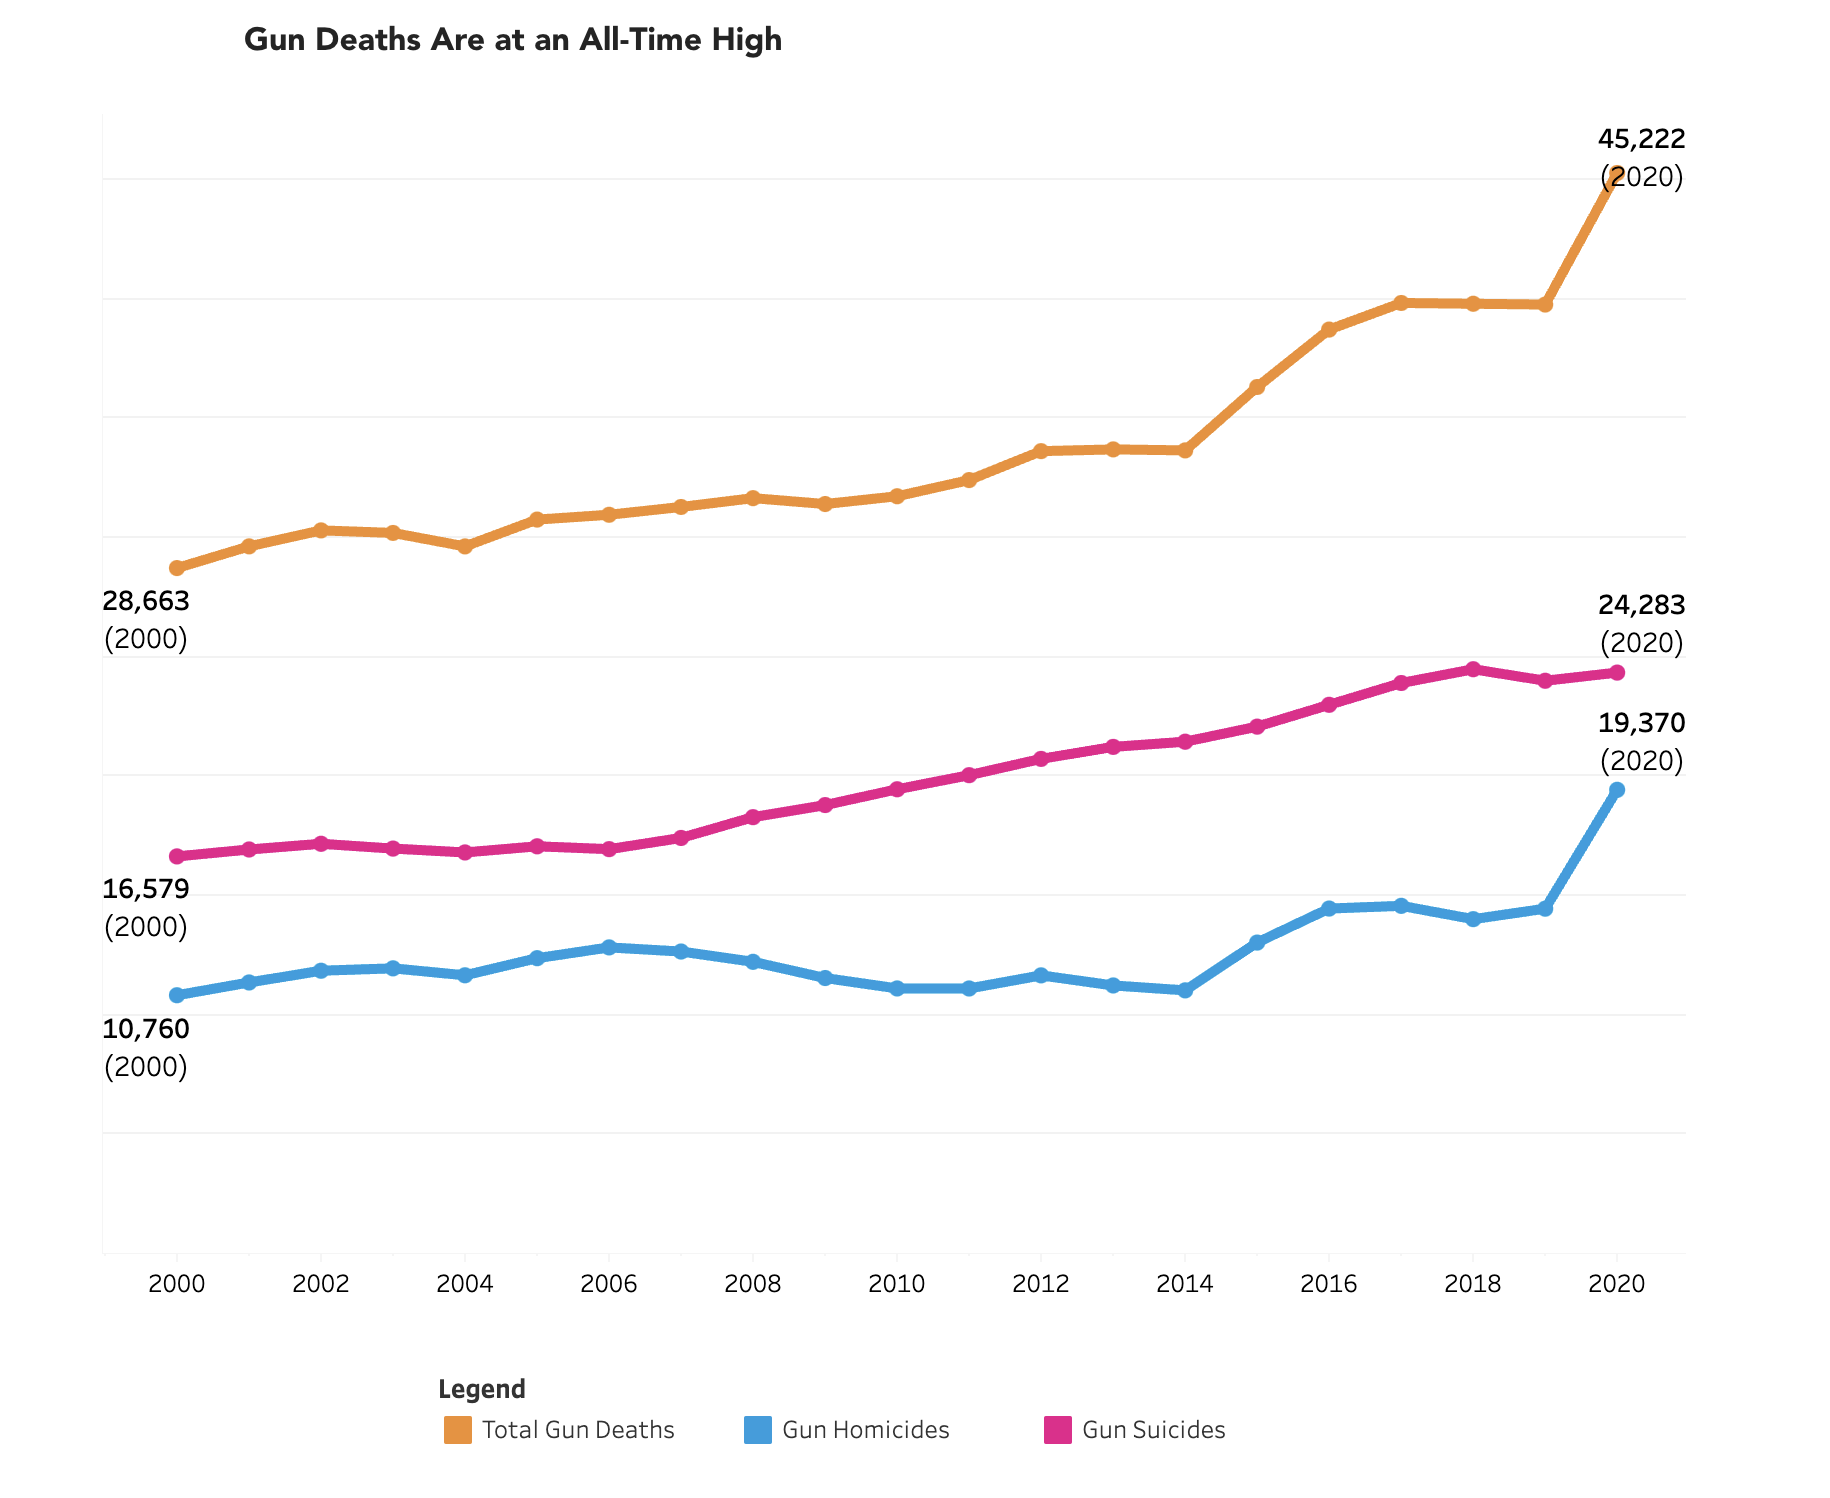
\includegraphics[width=0.8\textwidth]{st5442_assignment4/fig-extra-credit/Gun-deaths-are-at-an-all-time-high.png}
    \caption{
        Gun Deaths Are at an All-Time High \url{https://rockinst.org/blog/insights-from-the-gun-violence-data-dashboard/}
    }
    \label{fig:fig1}
\end{figure}

\section{Introduction}

For this analysis, I have chosen The Rockefeller Institute's Gun Violence Data Dashboard \cite{gun_violence_dashboard}, an interactive visualization that highlights firearm mortality trends across the United States. By employing a compelling narrative structure and persuasive techniques, it advocates for stricter gun control policies. Framing the data within a twenty-year context, it underscores the alarming spike in gun deaths in 2020, juxtaposed with earlier periods of relative stability.

\section{Analysis of Visualization Elements}

\subsection{Narrative Structure and Persuasive Techniques}

The dashboard's narrative is structured to emphasize the rise in gun-related fatalities, particularly homicides, which saw a record-breaking increase in 2020. This focus on year-over-year trends ties societal stressors, such as the COVID-19 pandemic, to the escalation of violence. Its segmentation of data by region, state, and demographic groups personalizes the issue, making the statistics relatable to diverse audiences. By highlighting the Northeast’s comparatively lower firearm mortality rates alongside stricter gun laws, the visualization implicitly suggests the effectiveness of legislative measures.

\subsection{Visual Elements Supporting the Message}

Visual elements like heat maps, line graphs, and bar charts effectively convey complex trends. For example, states with the highest firearm mortality rates are highlighted in bold gradients, drawing immediate attention. The use of color intensities and clear labels fosters accessibility while creating a sense of urgency. Regional comparisons are particularly impactful, showcasing stark contrasts in mortality rates and emphasizing the role of policy differences.

\begin{figure}[ht] % Change the position of your figure https://www.overleaf.com/learn/latex/Positioning_images_and_tables
    \centering
    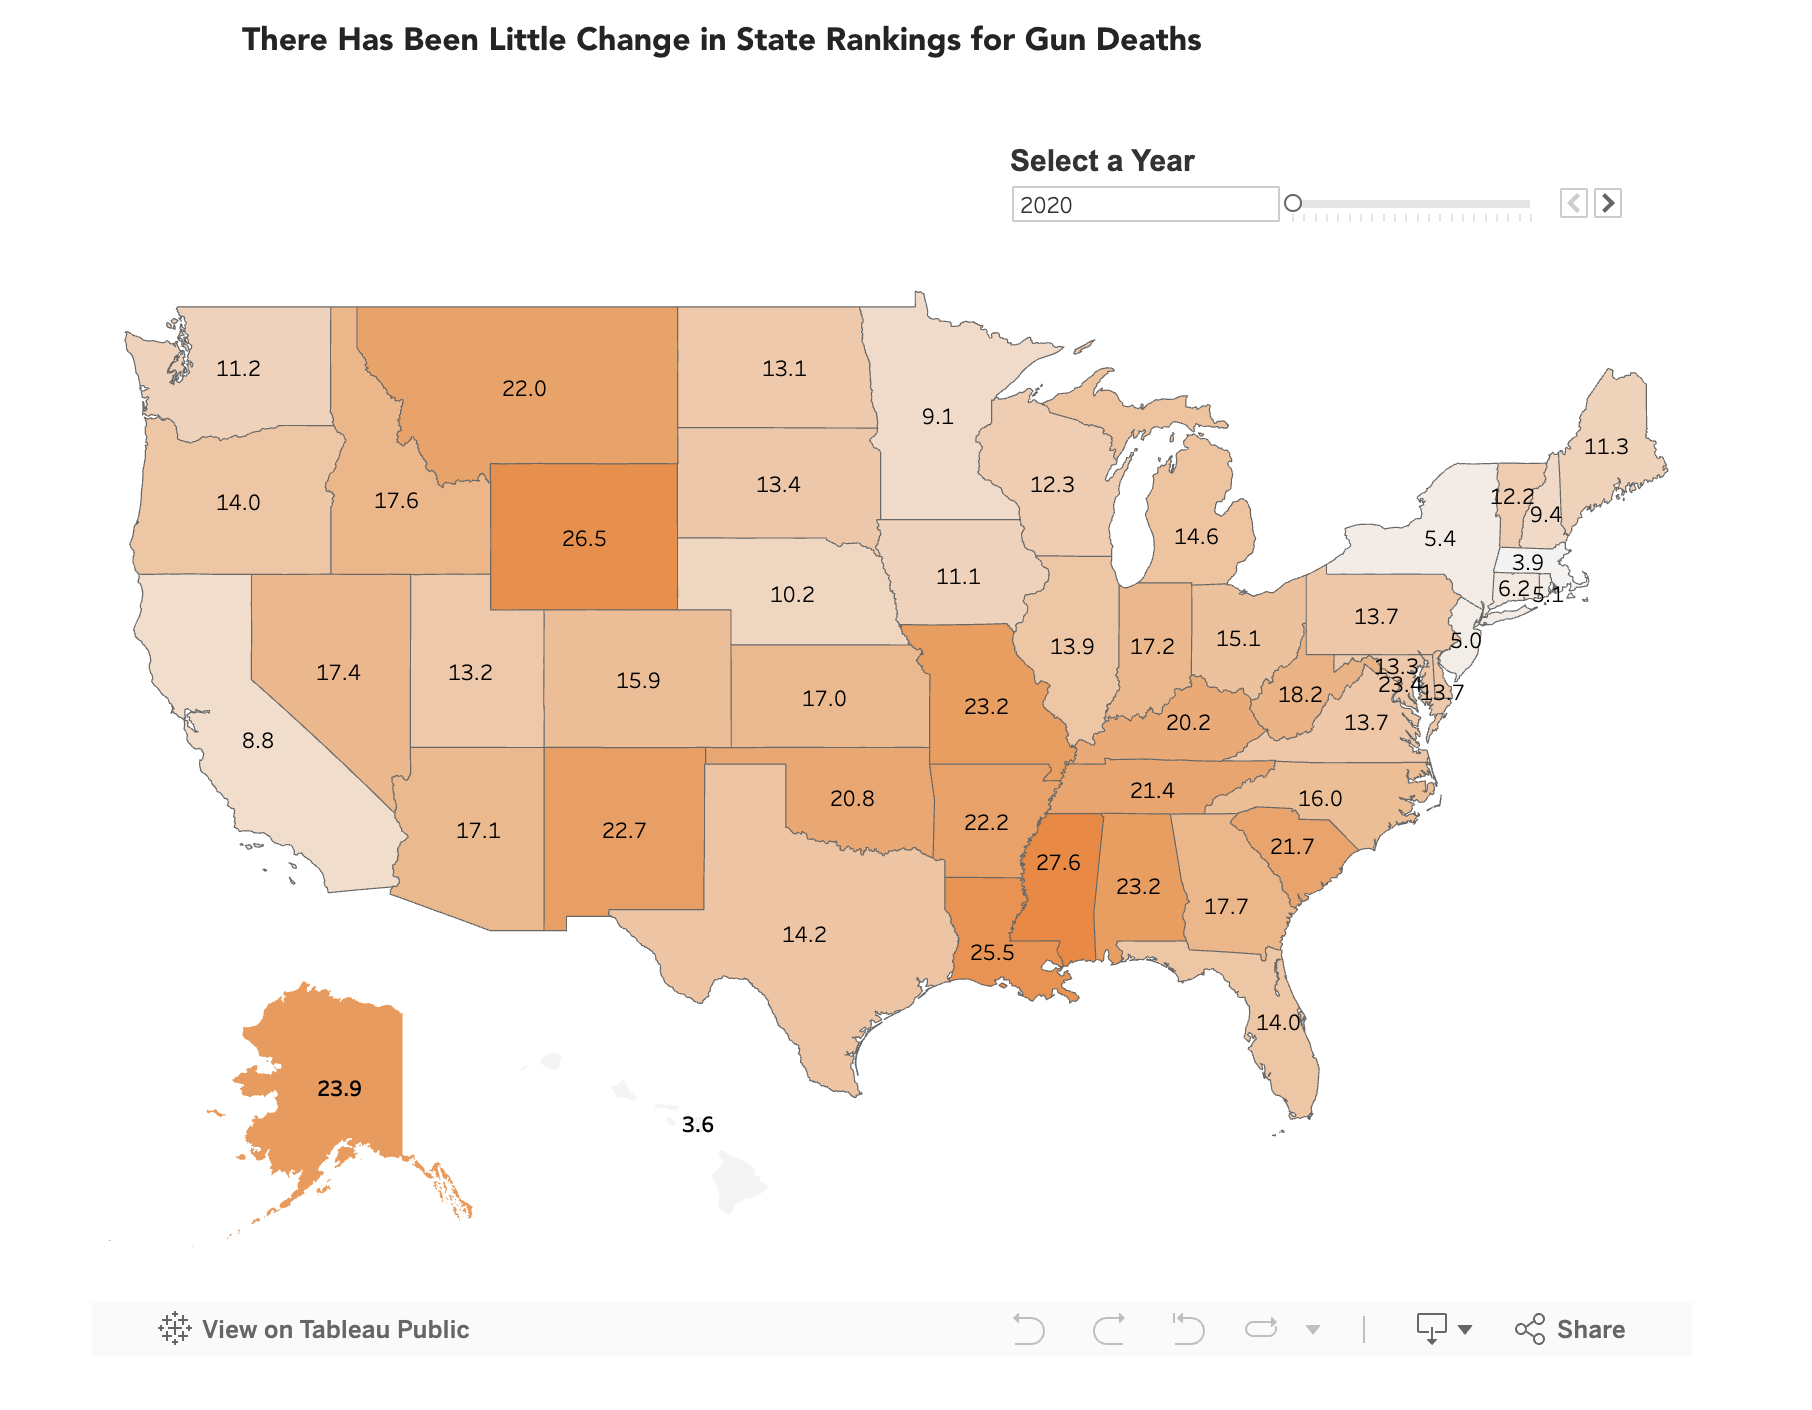
\includegraphics[width=0.8\textwidth]{st5442_assignment4/fig-extra-credit/state-rankings-gun-death.png}
    \caption{
        State Rankings for Gun Deaths \url{https://rockinst.org/blog/insights-from-the-gun-violence-data-dashboard/}
    }
    \label{fig:fig1}
\end{figure}

\subsection{Effectiveness of the Call to Action} 
While the dashboard does not explicitly propose solutions, its framing functions as an implicit call to action, encouraging policymakers to adopt stricter gun control measures. The detailed breakdowns of regional trends and demographic disparities support this advocacy, subtly reinforcing the need for intervention.

\subsection{Ethical Concerns} 
An ethical concern arises from the emphasis on absolute numbers without fully addressing socioeconomic or contextual factors, which may oversimplify causations. However, the dashboard adheres to ethical standards by relying on reputable sources like the CDC and avoiding sensationalism, ensuring its advocacy remains credible.

\section{Conclusion}

In summary, The Rockefeller Institute's Gun Violence Data Dashboard is a powerful tool for social advocacy. Its structured narrative, compelling visuals, and data-driven insights effectively convey the urgency of addressing gun violence, making it a persuasive resource for policy change.

\begin{refcontext}[sorting=nyt]
\printbibliography
\end{refcontext}

\end{document}

